\chapter{Technical Documents}
\label{ch:appendix_a}

% --- Database Schema Image ---
\begin{figure}[H]
    \centering
    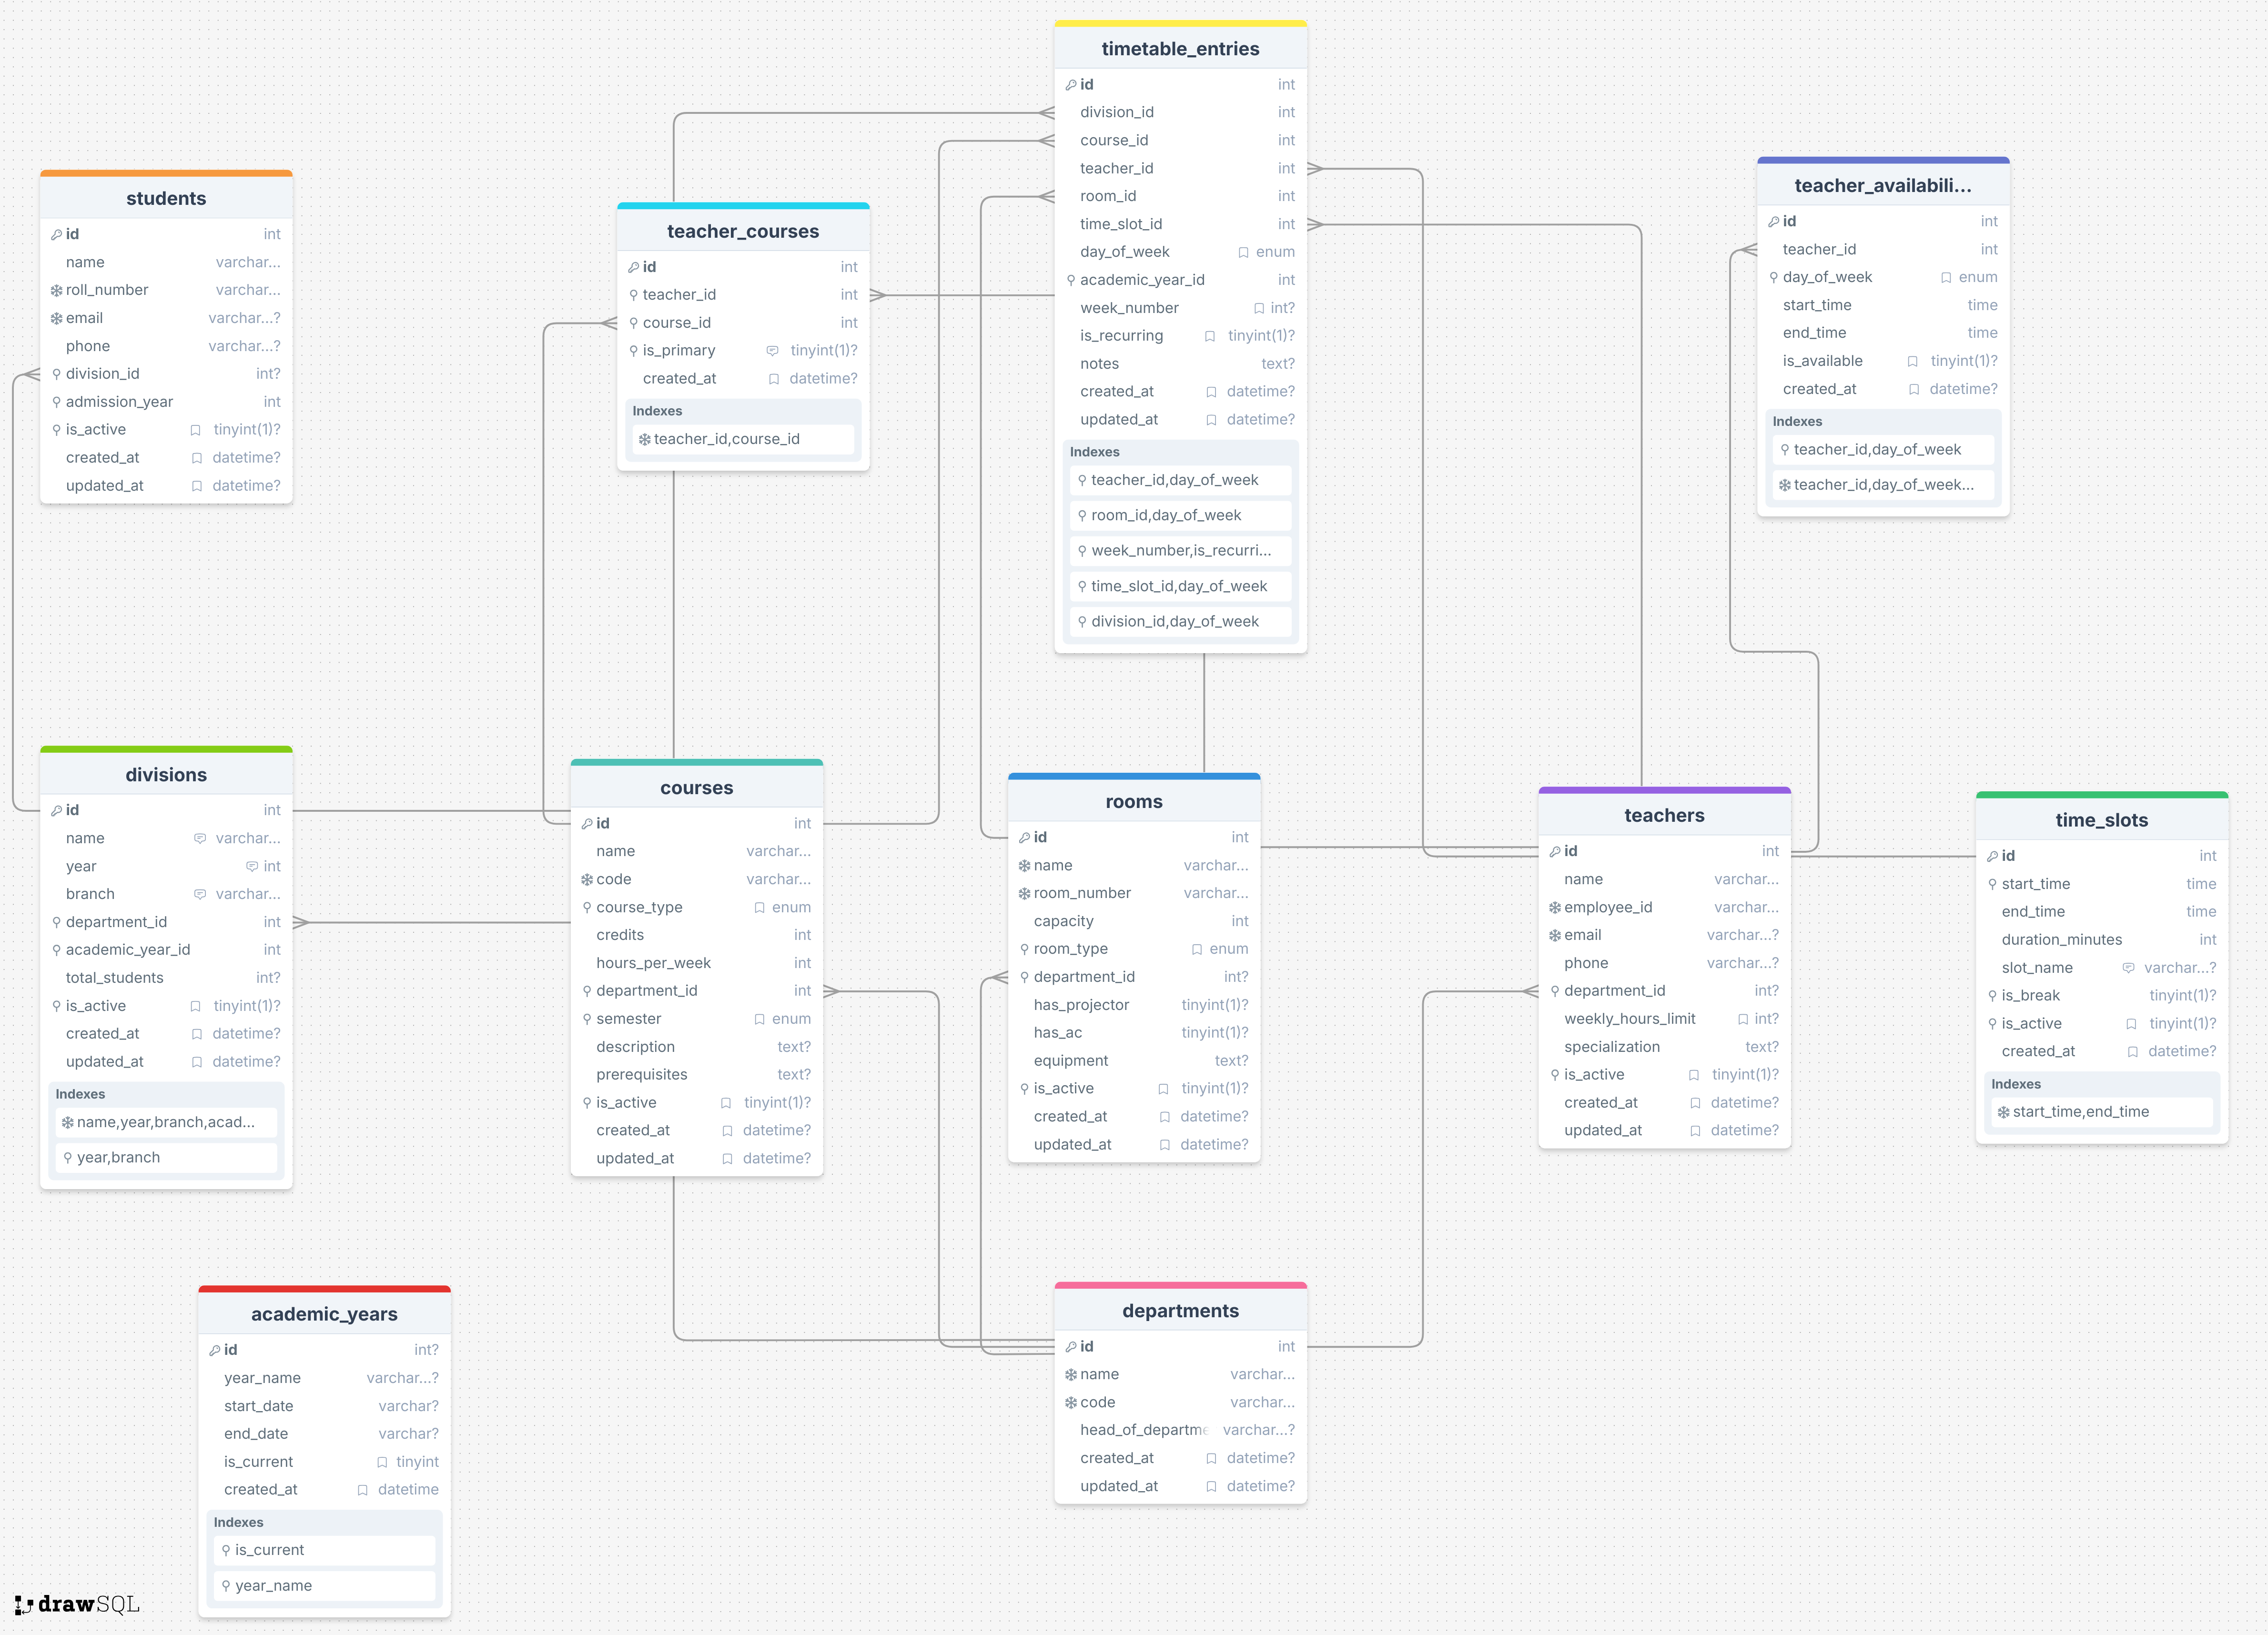
\includegraphics[width=1.12\linewidth]{schema_sql.png}
    \caption{SamaySetu Database Schema (Entity-Relationship View)}
    \label{fig:db_schema}
\end{figure}

\section{Data Dictionary}
The following tables describe the principal database entities used in the SamaySetu system. Entity classes live in the Java package \texttt{com.College.timetable.Entity}, and their corresponding SQL tables are created by Hibernate's JPA mapping.

\subsection{Table: \texttt{academic\_years}}
The top-level scoping entity. Every department, division, and timetable entry belongs to exactly one academic year.

\begin{table}[H]
    \centering
    \renewcommand{\arraystretch}{1.5}
    \begin{tabular}{|p{3.2cm}|p{2.5cm}|p{7.8cm}|}
        \hline
        \textbf{Field Name} & \textbf{Data Type} & \textbf{Description} \\
        \hline
        id & BIGSERIAL (PK) & Unique identifier. \\
        \hline
        year\_name & VARCHAR(20) UQ & Session name, e.g.\ ``2025-26''. Unique across the table. \\
        \hline
        start\_date & DATE & First day of the academic year. \\
        \hline
        end\_date & DATE & Last day of the academic year. \\
        \hline
        is\_current & BOOLEAN & True for exactly one row at any time; enforced by service logic. \\
        \hline
        created\_at & TIMESTAMP & Creation timestamp. \\
        \hline
    \end{tabular}
    \caption{Data Dictionary --- \texttt{academic\_years}}
    \label{tab:dd_academic_years}
\end{table}

\subsection{Table: \texttt{departments}}
Academic departments, scoped per academic year so that the organisational structure can evolve across years without destructive updates.

\begin{table}[H]
    \centering
    \renewcommand{\arraystretch}{1.5}
    \begin{tabular}{|p{3.5cm}|p{2.5cm}|p{7.5cm}|}
        \hline
        \textbf{Field Name} & \textbf{Data Type} & \textbf{Description} \\
        \hline
        id & BIGSERIAL (PK) & Unique identifier. \\
        \hline
        name & VARCHAR(100) & Department name (e.g.\ Computer Engineering). \\
        \hline
        code & VARCHAR(10) & Short code (e.g.\ COMP, ENTC, MECH). \\
        \hline
        head\_of\_department & VARCHAR(100) & HOD name (free text). \\
        \hline
        years & VARCHAR & Comma-separated list of supported years, e.g.\ ``1,2,3,4''. \\
        \hline
        academic\_year\_id & FK → academic\_years & Scoping academic year. \\
        \hline
    \end{tabular}
    \caption{Data Dictionary --- \texttt{departments}}
    \label{tab:dd_departments}
\end{table}

\subsection{Table: \texttt{divisions}}
A division identifies a specific year--branch--section group within a department for a given academic year.

\begin{table}[H]
    \centering
    \renewcommand{\arraystretch}{1.5}
    \begin{tabular}{|p{3.5cm}|p{2.5cm}|p{7.5cm}|}
        \hline
        \textbf{Field Name} & \textbf{Data Type} & \textbf{Description} \\
        \hline
        id & BIGSERIAL (PK) & Unique identifier. \\
        \hline
        name & VARCHAR(10) & Division label (A, B, SY-A, etc.). \\
        \hline
        year & INTEGER (1-4) & 1=FY, 2=SY, 3=TY, 4=BTech. \\
        \hline
        branch & VARCHAR(50) & Branch name. \\
        \hline
        total\_students & INTEGER & Strength; used by room-capacity conflict check. \\
        \hline
        time\_slot\_type & VARCHAR(20) & TYPE\_1 or TYPE\_2; selects the daily rhythm. \\
        \hline
        class\_teacher & VARCHAR(100) & Designated class teacher (free text). \\
        \hline
        department\_id & FK & Owning department. \\
        \hline
        academic\_year\_id & FK & Scoping academic year. \\
        \hline
    \end{tabular}
    \caption{Data Dictionary --- \texttt{divisions}}
    \label{tab:dd_divisions}
\end{table}

\subsection{Table: \texttt{courses}}
Theory and laboratory courses offered by departments.

\begin{table}[H]
    \centering
    \renewcommand{\arraystretch}{1.5}
    \begin{tabular}{|p{3cm}|p{3cm}|p{7.5cm}|}
        \hline
        \textbf{Field Name} & \textbf{Data Type} & \textbf{Description} \\
        \hline
        id & BIGSERIAL (PK) & Unique identifier. \\
        \hline
        name & VARCHAR(100) & Course name. \\
        \hline
        code & VARCHAR(20) UQ & Course code (e.g.\ CS201). \\
        \hline
        course\_type & ENUM & THEORY or LAB. \\
        \hline
        credits & INTEGER & Credit weight. \\
        \hline
        hours\_per\_week & INTEGER & Expected weekly teaching hours. \\
        \hline
        semester & ENUM & SEM\_1 .. SEM\_8. \\
        \hline
        year & INTEGER & 1-4 academic year. \\
        \hline
        department\_id & FK & Owning department. \\
        \hline
    \end{tabular}
    \caption{Data Dictionary --- \texttt{courses}}
    \label{tab:dd_courses}
\end{table}

\subsection{Table: \texttt{classrooms}}
Physical spaces: classrooms, laboratories, and auditoriums.

\begin{table}[H]
    \centering
    \renewcommand{\arraystretch}{1.5}
    \begin{tabular}{|p{3cm}|p{3cm}|p{7.5cm}|}
        \hline
        \textbf{Field Name} & \textbf{Data Type} & \textbf{Description} \\
        \hline
        id & BIGSERIAL (PK) & Unique identifier. \\
        \hline
        name & VARCHAR(50) UQ & Human-readable name. \\
        \hline
        room\_number & VARCHAR(20) UQ & Room code, e.g.\ H202. \\
        \hline
        building\_wing & VARCHAR(10) & Wing letter (auto-synced with the room number prefix). \\
        \hline
        capacity & INTEGER & Seating capacity. \\
        \hline
        room\_type & ENUM & CLASSROOM / LAB / AUDITORIUM. \\
        \hline
        has\_projector, has\_ac & BOOLEAN & Facility flags. \\
        \hline
        department\_id & FK (nullable) & Owning department, null if shared. \\
        \hline
    \end{tabular}
    \caption{Data Dictionary --- \texttt{classrooms}}
    \label{tab:dd_classrooms}
\end{table}

\subsection{Table: \texttt{time\_slots}}
Weekly time slots including break periods, organised as two profiles (TYPE\_1 and TYPE\_2).

\begin{table}[H]
    \centering
    \renewcommand{\arraystretch}{1.5}
    \begin{tabular}{|p{3cm}|p{3cm}|p{7.5cm}|}
        \hline
        \textbf{Field Name} & \textbf{Data Type} & \textbf{Description} \\
        \hline
        id & BIGSERIAL (PK) & Unique identifier. \\
        \hline
        start\_time, end\_time & TIME & Slot boundaries. \\
        \hline
        duration\_minutes & INTEGER & Used by the weekly-hour conflict check. \\
        \hline
        slot\_name & VARCHAR(50) & E.g.\ ``Period 1'', ``Lunch Break''. \\
        \hline
        is\_break & BOOLEAN & If true, entries are rejected in this slot. \\
        \hline
        type & VARCHAR(20) & TYPE\_1 or TYPE\_2. \\
        \hline
    \end{tabular}
    \caption{Data Dictionary --- \texttt{time\_slots}}
    \label{tab:dd_time_slots}
\end{table}

\subsection{Table: \texttt{users} (entity \texttt{TeacherEntity})}
A unified table for all authenticated users, regardless of role.

\begin{table}[H]
    \centering
    \renewcommand{\arraystretch}{1.5}
    \begin{tabular}{|p{3.5cm}|p{2.8cm}|p{7.2cm}|}
        \hline
        \textbf{Field Name} & \textbf{Data Type} & \textbf{Description} \\
        \hline
        id & BIGSERIAL (PK) & Unique identifier. \\
        \hline
        name & VARCHAR(100) & Full name. \\
        \hline
        employee\_id & VARCHAR(20) UQ & Institutional employee code. \\
        \hline
        email & VARCHAR UQ & Primary login identifier. \\
        \hline
        phone & VARCHAR(15) & Contact number. \\
        \hline
        min\_weekly\_hours & INTEGER & Minimum weekly teaching load. \\
        \hline
        max\_weekly\_hours & INTEGER & Upper cap enforced by conflict engine. \\
        \hline
        password & VARCHAR & BCrypt-hashed. \\
        \hline
        role & VARCHAR & ADMIN / HOD / TIMETABLE\_COORDINATOR / TEACHER. \\
        \hline
        is\_active, is\_approved, is\_email\_verified, is\_first\_login & BOOLEAN & Account lifecycle flags. \\
        \hline
        verification\_token, password\_reset\_token & VARCHAR & Transient tokens. \\
        \hline
        failed\_login\_attempts, account\_locked\_until & INTEGER, TIMESTAMP & Brute-force defence. \\
        \hline
        department\_id & FK (nullable) & Owning department (null for ADMIN). \\
        \hline
    \end{tabular}
    \caption{Data Dictionary --- \texttt{users}}
    \label{tab:dd_users}
\end{table}

\subsection{Table: \texttt{timetable\_entries}}
The core scheduling table. Each row represents one cell of the weekly grid for one division.

\begin{table}[H]
    \centering
    \renewcommand{\arraystretch}{1.5}
    \begin{tabular}{|p{3.8cm}|p{2.5cm}|p{7.2cm}|}
        \hline
        \textbf{Field Name} & \textbf{Data Type} & \textbf{Description} \\
        \hline
        id & BIGSERIAL (PK) & Unique identifier. \\
        \hline
        division\_id & FK → divisions & Division that owns this entry. \\
        \hline
        course\_id & FK → courses & Course being taught. \\
        \hline
        user\_id & FK → users & Teacher (note: column is \texttt{user\_id}, not \texttt{teacher\_id}). \\
        \hline
        classroom\_id & FK → classrooms & Room (note: column is \texttt{classroom\_id}). \\
        \hline
        time\_slot\_id & FK → time\_slots & Time slot. \\
        \hline
        day\_of\_week & ENUM & MONDAY .. SATURDAY. \\
        \hline
        academic\_year\_id & FK & Scoping academic year. \\
        \hline
        status & ENUM & DRAFT / PUBLISHED / ARCHIVED. \\
        \hline
        semester & ENUM (nullable) & SEM\_1 .. SEM\_8. \\
        \hline
        is\_lab\_session & BOOLEAN & True for lab entries. \\
        \hline
        batch\_id & FK (nullable) & For lab entries, the specific batch. \\
        \hline
        lab\_session\_group\_id & FK (nullable) & Ties sibling lab entries together. \\
        \hline
        notes & TEXT & Optional note. \\
        \hline
        created\_at, updated\_at & TIMESTAMP & Auto-maintained audit fields. \\
        \hline
    \end{tabular}
    \caption{Data Dictionary --- \texttt{timetable\_entries}}
    \label{tab:dd_timetable_entries}
\end{table}

\subsection{Table: \texttt{lab\_session\_groups}}
Parent row linking the $2 \times N$ child entries that together form one lab session.

\begin{table}[H]
    \centering
    \renewcommand{\arraystretch}{1.5}
    \begin{tabular}{|p{3.5cm}|p{2.5cm}|p{7.5cm}|}
        \hline
        \textbf{Field Name} & \textbf{Data Type} & \textbf{Description} \\
        \hline
        id & BIGSERIAL (PK) & Unique identifier. \\
        \hline
        division\_id & FK & Division being split into batches. \\
        \hline
        course\_id & FK & Lab course. \\
        \hline
        academic\_year\_id & FK & Scoping academic year. \\
        \hline
        day\_of\_week, time\_slot\_id & ENUM, FK & Starting slot of the two-period lab. \\
        \hline
        semester & ENUM (nullable) & Semester. \\
        \hline
        created\_by & FK → users & Administrator who created the session. \\
        \hline
    \end{tabular}
    \caption{Data Dictionary --- \texttt{lab\_session\_groups}}
    \label{tab:dd_lab_groups}
\end{table}

\subsection{Table: \texttt{user\_availability} (entity \texttt{TeacherAvailability})}
Optional per-slot availability preferences expressed by teachers.

\begin{table}[H]
    \centering
    \renewcommand{\arraystretch}{1.5}
    \begin{tabular}{|p{3.5cm}|p{2.5cm}|p{7.5cm}|}
        \hline
        \textbf{Field Name} & \textbf{Data Type} & \textbf{Description} \\
        \hline
        id & BIGSERIAL (PK) & Unique identifier. \\
        \hline
        user\_id & FK → users & The teacher. \\
        \hline
        day\_of\_week & ENUM & MONDAY .. SATURDAY. \\
        \hline
        start\_time, end\_time & TIME & Time window. \\
        \hline
        is\_available & BOOLEAN & True = free, False = unavailable. \\
        \hline
    \end{tabular}
    \caption{Data Dictionary --- \texttt{user\_availability}}
    \label{tab:dd_availability}
\end{table}

\newpage

\section{API Specifications}
The backend exposes RESTful endpoints under \texttt{http://<host>:8083}. Every non-\texttt{/auth/**} endpoint requires a JSON Web Token in the \texttt{Authorization: Bearer <jwt>} header.

\subsection{Authentication Module (\texttt{/auth})}
\begin{table}[H]
    \centering
    \renewcommand{\arraystretch}{1.4}
    \begin{tabular}{|p{1.8cm}|p{5.3cm}|p{6.5cm}|}
        \hline
        \textbf{Method} & \textbf{Endpoint} & \textbf{Description} \\
        \hline
        POST & \texttt{/auth/login} & Authenticate and receive JWT + role + firstLogin. \\
        \hline
        POST & \texttt{/auth/register} & Self-register using an MITAOE email. \\
        \hline
        GET & \texttt{/auth/verify-email} & Verify email via token from email. \\
        \hline
        POST & \texttt{/auth/forgot-password} & Request password-reset link. \\
        \hline
        POST & \texttt{/auth/reset-password} & Reset password using valid token. \\
        \hline
        POST & \texttt{/auth/change-first-password} & First-login password change. \\
        \hline
    \end{tabular}
    \caption{Authentication API Endpoints}
    \label{tab:api_auth}
\end{table}

\subsection{Staff Self-Service Module (\texttt{/api/staff})}
Accessible to all authenticated roles.
\begin{table}[H]
    \centering
    \renewcommand{\arraystretch}{1.4}
    \begin{tabular}{|p{1.8cm}|p{5.3cm}|p{6.5cm}|}
        \hline
        \textbf{Method} & \textbf{Endpoint} & \textbf{Description} \\
        \hline
        GET & \texttt{/api/staff/profile} & Retrieve own profile. \\
        \hline
        PUT & \texttt{/api/staff/profile} & Update own phone / specialization. \\
        \hline
        POST & \texttt{/api/staff/change-password} & Change own password. \\
        \hline
        GET & \texttt{/api/staff/availability} & Retrieve own availability rows. \\
        \hline
        PUT & \texttt{/api/staff/availability} & Replace availability (atomic). \\
        \hline
    \end{tabular}
    \caption{Staff API Endpoints}
    \label{tab:api_staff}
\end{table}

\subsection{Teacher Management Module (\texttt{/api/teachers})}
\begin{table}[H]
    \centering
    \renewcommand{\arraystretch}{1.4}
    \begin{tabular}{|p{1.8cm}|p{5.3cm}|p{6.5cm}|}
        \hline
        \textbf{Method} & \textbf{Endpoint} & \textbf{Description} \\
        \hline
        GET & \texttt{/api/teachers} & List all teachers. \\
        \hline
        GET & \texttt{/api/teachers/\{id\}} & Single teacher by ID. \\
        \hline
        GET & \texttt{/api/teachers/pending-approvals} & Queue of self-registrations. \\
        \hline
        POST & \texttt{/api/teachers/\{id\}/approve} & Approve a pending teacher. \\
        \hline
        POST & \texttt{/api/teachers/\{id\}/reject} & Reject with reason. \\
        \hline
    \end{tabular}
    \caption{Teacher Admin API Endpoints}
    \label{tab:api_teacher}
\end{table}

\subsection{Administrative Master-Data (\texttt{/admin/api/})}
Restricted to ADMIN / HOD / TIMETABLE\_COORDINATOR.
\begin{table}[H]
    \centering
    \renewcommand{\arraystretch}{1.4}
    \begin{tabular}{|p{3.2cm}|p{4.5cm}|p{6.5cm}|}
        \hline
        \textbf{Resource} & \textbf{Endpoint Suffix} & \textbf{Supported Operations} \\
        \hline
        Academic Years & \texttt{../academic-years} & GET List/ID/Current, POST, PUT, DELETE \\
        \hline
        Departments & \texttt{../departments} & GET List/ID/ByYear, POST, PUT, DELETE, POST copy \\
        \hline
        Courses & \texttt{../courses} & GET List/ID, POST, PUT, DELETE \\
        \hline
        Divisions & \texttt{../divisions} & GET List/ID/ByYear, POST, PUT, DELETE \\
        \hline
        Batches & \texttt{../batches} & GET List/ID/ByDivision, POST, PUT, DELETE \\
        \hline
        Rooms & \texttt{../rooms} & GET List/ID, POST, PUT, DELETE \\
        \hline
        Time Slots & \texttt{../time-slots} & GET List/ID/Active/ByType, POST, PUT, DELETE \\
        \hline
    \end{tabular}
    \caption{Admin CRUD Endpoints}
    \label{tab:api_admin_crud}
\end{table}

\subsection{Timetable Module (\texttt{/api/timetable})}
\begin{table}[H]
    \centering
    \renewcommand{\arraystretch}{1.4}
    \begin{tabular}{|p{1.8cm}|p{5.3cm}|p{6.5cm}|}
        \hline
        \textbf{Method} & \textbf{Endpoint} & \textbf{Description} \\
        \hline
        GET & \texttt{../division/\{id\}} & Published timetable for a division (cached). \\
        \hline
        GET & \texttt{../teacher/\{id\}} & Published timetable for a teacher (cached). \\
        \hline
        GET & \texttt{../draft} & Draft entries for admin review. \\
        \hline
        GET & \texttt{../validate} & Pre-publish validation result. \\
        \hline
        POST & \texttt{../entries} & Create entry (conflict-checked). \\
        \hline
        PUT & \texttt{../entries/\{id\}} & Update / move (conflict-checked). \\
        \hline
        DELETE & \texttt{../entries/\{id\}} & Delete entry. \\
        \hline
        DELETE & \texttt{../draft} & Clear all DRAFT entries for a division. \\
        \hline
        POST & \texttt{../lab-session} & Atomic lab-session creation via wizard. \\
        \hline
        DELETE & \texttt{../lab-groups/\{id\}} & Cascade delete a lab session group. \\
        \hline
        POST & \texttt{../copy} & Copy DRAFT entries between divisions. \\
        \hline
        POST & \texttt{../publish} & Publish draft (archives previous version). \\
        \hline
        POST & \texttt{../archive} & Archive currently-published timetable. \\
        \hline
        GET & \texttt{../export/division/\{id\}/pdf} & Download division PDF. \\
        \hline
        GET & \texttt{../export/division/\{id\}/excel} & Download division Excel. \\
        \hline
        GET & \texttt{../export/teacher/\{id\}/pdf} & Download teacher PDF. \\
        \hline
        GET & \texttt{../export/teacher/\{id\}/excel} & Download teacher Excel. \\
        \hline
    \end{tabular}
    \caption{Timetable API Endpoints}
    \label{tab:api_timetable}
\end{table}

\subsection{Admin Bulk Operations (\texttt{/admin})}
Restricted to ADMIN.
\begin{table}[H]
    \centering
    \renewcommand{\arraystretch}{1.4}
    \begin{tabular}{|p{1.8cm}|p{5.3cm}|p{6.5cm}|}
        \hline
        \textbf{Method} & \textbf{Endpoint} & \textbf{Description} \\
        \hline
        POST & \texttt{/admin/upload-staff} & Bulk staff CSV upload. \\
        \hline
        POST & \texttt{/admin/create-staff} & Create a single staff member. \\
        \hline
        GET & \texttt{/admin/download-staff-template} & Download the CSV template. \\
        \hline
        PUT & \texttt{/admin/update-staff/\{id\}} & Admin-level staff update. \\
        \hline
        POST & \texttt{/admin/upload-courses} & Bulk course CSV upload per dept + year. \\
        \hline
        GET & \texttt{/admin/download-courses-template} & Download course CSV template. \\
        \hline
    \end{tabular}
    \caption{Admin Bulk-Operation Endpoints}
    \label{tab:api_admin_bulk}
\end{table}

\section{Deployment Configuration Summary}

\subsection{Development Profile (\texttt{application-dev.properties})}
\begin{itemize}
    \item Database: PostgreSQL 17 at \texttt{localhost:5432/SamaySetu}
    \item Redis: \texttt{localhost:6379} (Memurai on Windows, redis-server on Linux/macOS)
    \item JWT secret: shipped Base64 default
    \item Email: Gmail SMTP at \texttt{smtp.gmail.com:587}
    \item \texttt{ddl-auto=update}; SQL logging at DEBUG
    \item Default admin: \texttt{suryankadmin@mitaoe.ac.in} / \texttt{Admin@123}
    \item Staff default password: \texttt{mitaoe@123} for testing
\end{itemize}

\subsection{Production Profile (\texttt{application-prod.properties})}
\begin{itemize}
    \item Database: AWS RDS PostgreSQL (URL from \texttt{SPRING\_DATASOURCE\_URL})
    \item Redis: Managed service (ElastiCache) with in-transit TLS
    \item JWT secret: \texttt{JWT\_SECRET\_KEY} env variable only; no default
    \item \texttt{ddl-auto=validate}; SQL logging at WARN
    \item All secrets loaded from environment; no file-based defaults
    \item Staff default password: \texttt{random} (UUID per staff member)
    \item CORS allowed origins: AWS Amplify frontend domain
\end{itemize}
